\documentclass[10pt,compress,mathserif]{beamer}
\usetheme{Singapore}
% Few theme names Berkeley Copenhagen Dresden


\usepackage{amsmath,minibox,amssymb,amsfonts,amsthm,graphicx,color,multirow,array,tikz,hyperref}
\usetikzlibrary{arrows,snakes,backgrounds,patterns,matrix,shapes,fit,calc,shadows, positioning}

\setbeamertemplate{navigation symbols}{} % This is just to get rid of the extra fazool symbols
\setbeamerfont{caption}{size=\footnotesize}

\title[]{Circuit and Systems 1 Project}
\author[]{Salman Ahmed and Faiz Ullah\\ Section A DCSE \\ UET Peshawar.}
\rightskip=0pt plus 0pt

\begin{document}

\begin{frame}    \titlepage \end{frame}



% First slide
\section{Introduction}
\begin{frame}{Introduction to Project}
\noindent Introduce your project and problem statement. \\ \vskip10pt
Electricity is generated when a conductor is moved around a magnetic field. How to design a circuit to generate 12V electricity from a magnetic field.

\end{frame}



% Second Slide
\section{Solution}
\begin{frame}{Circuit Diagram}
Put your circuit diagram and calculations.
The state-space representation of the system can be written as follows:
\begin{figure}[h!]
\centering
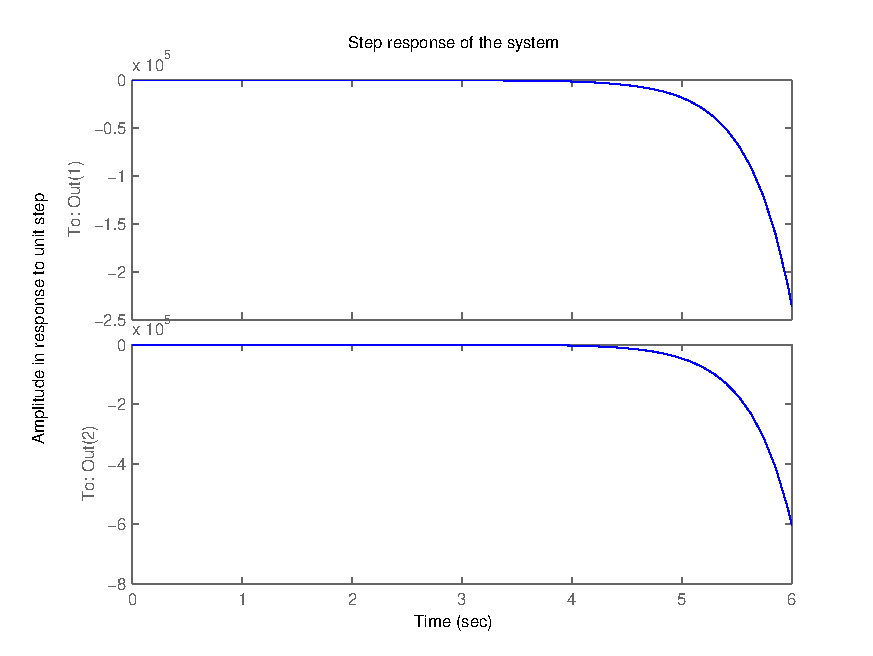
\includegraphics[scale=0.40]{Step_Res.pdf}
\caption{This is sample figure - put your circuit diagram.}
\end{figure}

\end{frame}


\section{Circuit Analysis}
\begin{frame}{Circuit Analysis}
Put analysis that you perform in this slide. (Calculations of voltage and calculation of currents).
\end{frame}





\section{Results}
\begin{frame}{Results}
Put results that you obtain with pSpice and actual results.
\end{frame}



\end{document} 